\documentclass[conference]{IEEEtran}

% --- IDIOMA ---
\usepackage[spanish, es-tabla]{babel}

% --- FUENTES (XeLaTeX) ---
\usepackage{fontspec}
\setmainfont{Liberation Serif}
\setmonofont{JetBrainsMono Nerd Font}

% --- CITAS IEEE ---
\usepackage[backend=biber,style=ieee,sorting=none]{biblatex}
\addbibresource{referencias.bib}

% --- UTILIDADES ---
\usepackage{graphicx}
\usepackage{float}
\usepackage{amsmath}
\usepackage{booktabs}
\usepackage[colorlinks=true,linkcolor=black,citecolor=black,urlcolor=blue]{hyperref}

% --- CÓDIGO ---
\usepackage{xcolor}
\definecolor{bg}{RGB}{40,44,52}

\usepackage{minted}

\setminted{
  style=monokai,
  bgcolor=bg,
  breaklines,
  breakanywhere=true,
  tabsize=2,
  fontsize=\footnotesize
}

\usepackage{csquotes}

\begin{document}



% --- INICIO DE LA PORTADA ---
\begin{titlepage}
    \centering
    \vspace*{0.5cm}
    
    % --- Escudo de la UV ---
    % Asegúrese de tener el archivo "escudo_uv.png" (o .jpg) en su carpeta del proyecto
    
\includegraphics[width=0.3\textwidth]{UV.png} \\ 
    \vspace{0.8cm}
    
    {\huge \textbf{Universidad Veracruzana}} \\
    \vspace{0.4cm}
    {\Large Facultad de Instrumentación Electrónica} \\ % Corregido: Instrumentación
    \vspace{0.2cm}
    {\large Ingeniería Biomédica} \\
    
    \vfill
    
    % Título de la Experiencia Educativa y Actividad
    {\Large \textbf{EE: Interfaces Hombre-Máquina}} \\
    \vspace{0.8cm}
    {\Large \textbf{ACTIVIDAD 04. SENSOR INERCIAL MPU6050 COMO DISPOSITIVO PARA UNA INTERFAZ HOMBRE-MAQUINA}} \\
    
    \vspace{1.5cm}
 
    % Información de los Integrantes
    \begin{flushright} % Alineado a la derecha para un toque más profesional
        \textbf{Profesor:} \\
        Varela Lara Luis Julian \\
        \vspace{0.5cm}
        \textbf{Integrantes del equipo ``\textit{ES3.14}}'': \\
        Alfonso Gamboa Rubén \\
        Flores Montero Edsel Yetlanezi \\
    \end{flushright}
    
    \vfill
    
    {\large \textbf{Fecha:} 29 de abril de 2026} \\
    \vspace{1cm}
    {\small Xalapa, Enríquez, Ver.} % O la sede correspondiente
\end{titlepage}
% --- FIN DE LA PORTADA ---



% --- EL CUERPO DEL TEXTO (Automáticamente en dos columnas) ---

\section{Introducción al tema.}
El siguiente reporte incluye la información empleada para la construcción, explica la lógica del control y la integración de los dispositivos MPU6050 \cite{invensense2013mpu6050} y el microcontrolador ESP32 con el objetivo de establecer un sistema físico (Hardware) inalámbrico que permita interactuar en tiempo real con el programa ``ComandosRS232''.

\section{Marco teórico}

  \subsection{ESP32 Microcontrolador.}
  El ESP32 DevKit V1 cuenta con conectividad inalámbrica nativa y opera a altas frecuencias, esto permite el procesamiento de señales digitales (DSP, por sus siglas en inglés) en tiempo real, facilitando la lectura de sensores y la transmisión de datos con baja latencia. \cite{espressif2023esp32}
  \subsection{Comunicación}
  Bluetooth Serial (SPP): Es un estándar de comunicación inalámbrica que emula el perfil de puerto serie tradicional. Este el intercambio de datos entre el microcontrolador y la computadora, funcionando de manera qué simula a la comunicación física, pero eliminando la restricción de los cables para otorgar total libertad de movimiento a la interfaz.
  \subsection{Sensor Inercial MPU6050}
  El MPU6050 es un dispositivo microelectromecánico (MEMS) de 6 grados de libertad (6DOF, por sus siglas en inglés) enfocado en la captura de movimiento para interfaces hombre-máquina (HMI). Está compuesto internamente por un acelerómetro de 3 ejes y un giroscopio de 3 ejes en una sola pastilla de silicio. \cite{invensense2013mpu6050}
  \paragraph{Funcionamiento} El voltaje de operación compatible oscila entre 3.3V y 5V DC, por lo qué se puede conectar a cualquiera de los pines del ESP32, ya sea en 3.3V y el VIN. Se comunica con el microcontrolador a través de protocolo I2C (Inter-Integrated Circuit). 
  Internamente, el acelerómetro mide la aceleración estática (fuerza de gravedad) y dinámica en los ejes X, Y, y Z. Descomponiendo estos vectores, es posible calcular los ángulos de inclinación (Pitch y Roll) de la mano. Por su parte, el giroscopio mide la velocidad angular en grados por segundo, lo que resulta fundamental para detectar rotaciones abruptas o cambios rápidos de posición que el acelerómetro no puede filtrar adecuadamente.

\section{Dearrollo de la actividad.}
  \subsection{Adquisición de Datos y Hardware}
  Para el desarrollo de esta actividad se usaron únicamente los ascelerómtros del sensor GPU6050, cuales el ESP32 obtiene mediante el protocolo $I^2C$ y la librería \textit{Adafrui MPU6050} \cite{adafruit2021mpu6050}. Para optimizar la lectura enfocada en movimientos humanos, el sensor se configuró con un rango de aceleración de ±8g y un filtro paso bajo (Bandwidth) de 21 Hz, lo que elimina de antemano vibraciones de alta frecuencia que no provienen de la mano.

  \subsection{Procesamiento Matemático y Filtrado}
  Los datos crudos del acelerómetro no pueden usarse directamente como comandos debido a la gravedad y al ruido del sensor. Por ello en la parte del código ``Fase de calibración''.

  \subsection{Calibración Dinámica y Concurrencia}
  Uno de los mayores retos en la programación de microcontroladores para tiempo real es evitar el bloqueo del procesador. El código fue diseñado bajo un paradigma "no bloqueante", sustituyendo por completo la función delay() por el temporizador interno del sistema (millis()). Esto permite que el ESP32 evalúe múltiples tareas simultáneamente: muestrear el sensor a 125 Hz, enviar datos por Bluetooth cada 24 ms, y ejecutar una rutina de calibración dinámica. Dicha calibración promedia 15 muestras iniciales para establecer un "punto cero" relativo a la postura natural de la mano del usuario, permitiendo que el dispositivo sea cómodo de usar en cualquier posición inicial.
  
  \subsection{Desarrollo del código.}
  
    \begin{figure}[t]
      \centering
      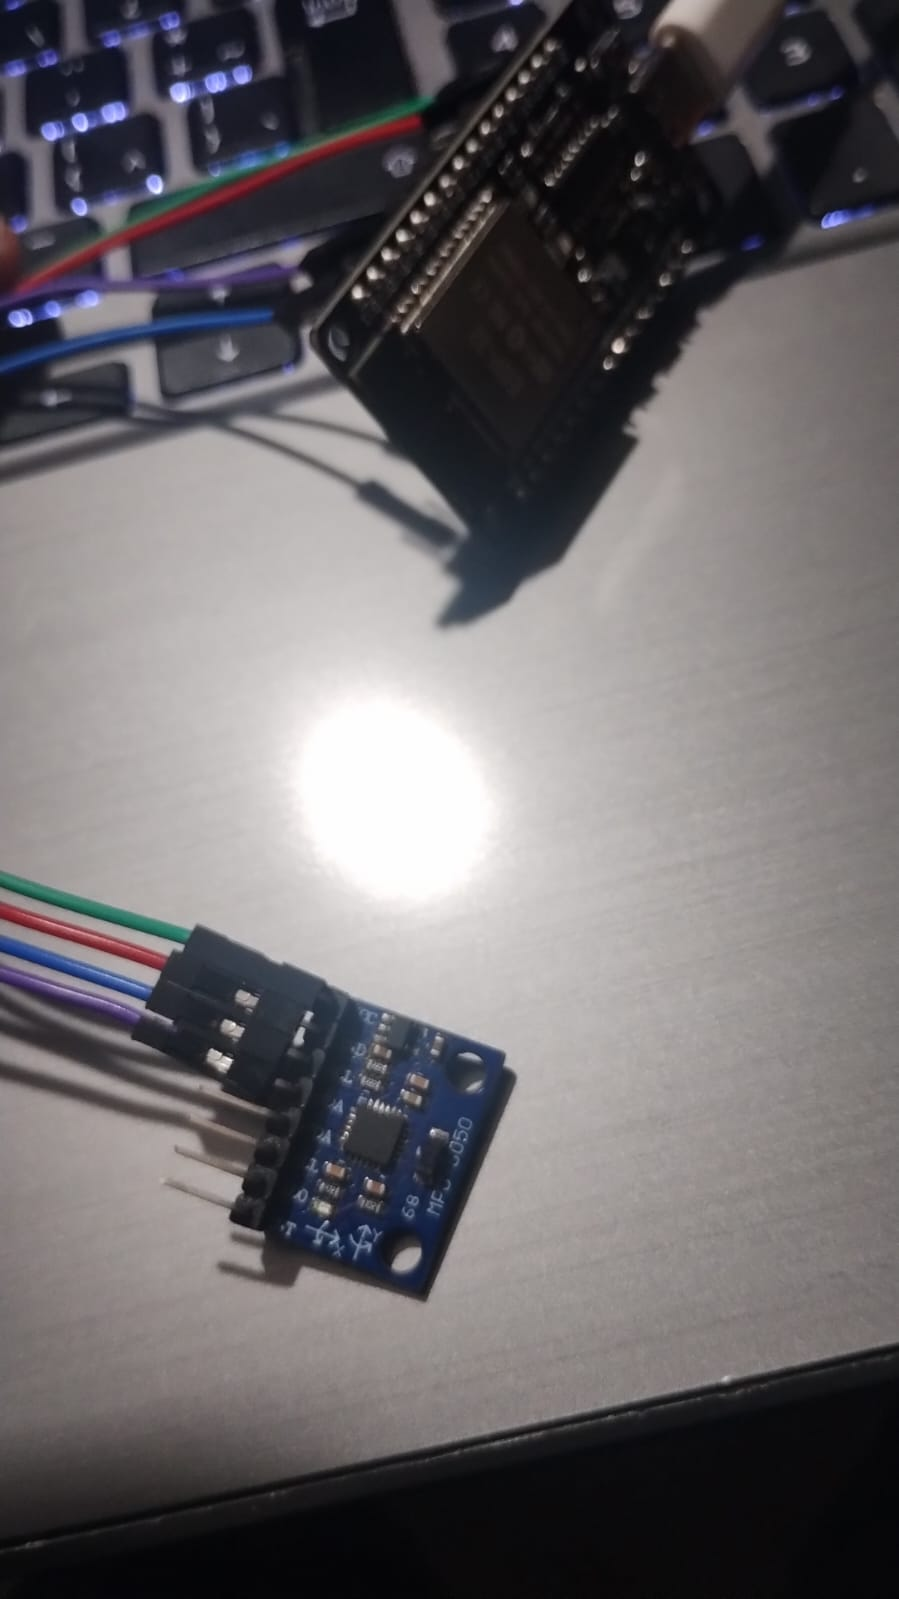
\includegraphics[width=\linewidth]{circuito.jpeg} % \linewidth se ajusta a la columna
      \caption{Conexiones con Jumpers hembra - hembra, conectando vcc con 3.3v; GND - GND; SDA - pin21; SCL - pin 22.}
      \label{fig:circuito}
    \end{figure}

  \subsection{Conexiones y pines}
  
  
  Podemos apreciar las concexiones físicas en la figura \ref{fig:circuito} \\ \\ 
  \textbf{Pines declarados en el código:} \\
  \begin{itemize}
    \item GND (Ground): Tierra
    \item VCC: DC (3.3V - 5V)
    \item SDA (Serial Data): Línea de datos bidireccional I2C.
    \item Pin digital 21.SCL (Serial Clock): Línea de reloj I2C.
    \item Pin digital 22.Diseño del sistemaInterconexión.
    \item MPU6050 - ESP32GND (Ground) MPU6050 - GND (Ground) ESP32VCC.
    \item MPU6050 - 3.3V / 5V ESP32SDA MPU6050 - Pin Digital 21 ESP32SCL.
    \item MPU6050 - Pin Digital 22 ESP32Botón de Calibración - Pin Digital 0 (BOOT).
    \item ESP32 (Activar: INPUT\_PULLUP)
  \end{itemize}

  \subsection{Diseño del Control}
  En esta sección se explica la información necesaria empleada para diseñar la interfaz Hombre-Máquina (HMI), la lógica empleada para el procesamiento digital de señales inerciales y su posterior incorporación en el código diseñado para controlar el programa ComandosRS232.

Para garantizar un análisis correcto de los movimientos de la mano y asegurar que las frecuencias de corte de los filtros digitales se respeten, se estableció una frecuencia de muestreo estricta de 125 Hz.

Para lograr esto sin bloquear el reloj del microcontrolador, se evitó por completo el uso de la función de retardo cíclico. En su lugar, se implementó un control asíncrono que evalúa el tiempo en milisegundos para garantizar que la lectura del sensor ocurra exactamente en el intervalo requerido (8 ms). Esto permite que la adquisición de datos, el filtrado y el envío de datos por Bluetooth (configurado a 24 ms, tres veces mayor a la frecuencia de muestreo) se ejecutan en hilos lógicos independientes sin interferencia mutua.

Dado que la posición prona natural "cero" varía según la anatomía de cada usuario y la colocación exacta del sensor en el dorso de la mano, el sistema requiere una calibración inicial. Al arrancar el dispositivo (o al presionar el botón BOOT integrado), el sistema toma un promedio de 15 muestras estáticas. Este valor promedio se convierte en el "offset" que se resta a todas las lecturas posteriores, estableciendo un origen de coordenadas dinámico y perfectamente adaptado a la postura de reposo del usuario.

Para evitar movimientos descontrolados del cursor causados por el temblor natural de la mano, se calcularon umbrales de activación mapeando una variable de "sensibilidad" (1-100) a un rango específico de grados de inclinación. Cualquier lectura que caiga por debajo de este umbral angular es considerada "Zona Muerta" (Velocidad Cero). 

Solo cuando el movimiento de la mano, ya sea de flexión, extensión, pronación o supinación superan este umbral definido por la zona muerta (positivo o negativo), se transmiten los comandos de dirección correspondientes. Las lecturas crudas del acelerómetro son altamente susceptibles a ruido de alta frecuencia y micro-vibraciones. Para aislar exclusivamente los movimientos suaves intencionales (baja frecuencia) que controlan la dirección del cursor, se implementó un filtro digital pasa bajos mediante una Media Móvil Exponencial (EMA). La ecuación que rige este comportamiento es:$$Y_n = (\alpha \times X_n) + ((1 - \alpha) \times Y_{n-1})$$Donde $Y_n$ es el ángulo filtrado, $X_n$ es la lectura cruda actual, y $\alpha$ es el factor de suavizado constante (0.10). Esto estabiliza la señal sacrificando una fracción de tiempo de respuesta, de lo contrario, la velocidad en la qué se percibe resultaría demasiado rápida en la pantalla. 

Para la sección "RECORTAR IMAGEN", se requiere identificar una acción de tipo "clic sostenido" mediante un movimiento abrupto y rápido. Dado que el filtro pasa bajos anterior elimina estas frecuencias, se optó por analizar la magnitud del vector tridimensional del giroscopio de forma independiente:$$|G| = \sqrt{Gx^2 + Gy^2 + Gz^2}$$. Si la magnitud de la velocidad angular supera la velocidad de rotación (alta frecuencia), se registra el evento de selección (enviando el comando 50). Para evitar que un solo movimiento abrupto genere múltiples "clics" indeseados (efecto rebote), se incorporó un tiempo de bloqueo (cooldown) de 700 ms, durante el cual se ignoran picos posteriores.

  \newpage
  \subsection{Código completo}
    A continuación se deja el código completo usado durante el desarrollo de esta actividad:
    \inputminted{cpp}{Act04.ino}



\section{Conclusiones}
  \subsection{Dificultades enfrentadas}
  Durante el desarrollo de esta actividad el equipo se enfrentó a varias dificultades técnicas tanto con el software como con el hardware:
  \paragraph{Migración de ESP32-S3 a ESP32 clásico} El desarrollo de la práctica se pensó inicialmente para la placa \textit{ESP32-S3}, pues se pensaba usar su capacidad de procesar vectores, conceptualizando como vectores con dirección y magnitud en los planos X y Y. Sin  embargo el \textit{ESP32-S3} opera exclusivamente con \textbf{Bluetooth Low Energy (BLE)}. Lo cual suponía un problema con la velocidad a la que se tenia que leer e imprimir los datos; migrando así a \textit{ESP32 clásico}.
  \paragraph{Sensibilidad} Para poder calibrar el cero de nuestro sensor y para la sensibilidad de este, se tuvieron que hacer unas variables que fungian como configuración, esto para poder realizar múltiples pruebas del código con ayuda del programa \textit{ComandosRS232} brindado por el profesor, que se determinó manualmente la sensibilidad adecuada junto con una velocidad de impresión cómoda brindado por el profesor, que se determinó manualmente la sensibilidad adecuada junto con una velocidad de impresión cómoda.
  \paragraph{Calibración} Como cada mano tiene un ángulo distinto, se tuvo que añadir una fase de calibración, que se encarga de tomar este ángulo natural para tratarlo como un cero durante el arranque del microcontrolador, para esto es necesario reiniciar la ESP32 para que se adapte a cada mano.
  \paragraph{Diagónistico de Sensor} Gran parte del desarrollo de la actividad fue en tratar de solucionar el \textit{¿Por qué el ESP32 no es capaz de leer al sensor?}, por loque se desarrolló un software para poder diagnosticar el estado del sensor, llegando a la conclusión de
  
  \subsection{Aprendizaje obtenido}
  Los aprendizajes adquiridos durante el desarrollo de la actividad fueron:
  \begin{itemize}
    \item Programación de un ESP32 con ayuda de Arduino-IDE, Arduino-cli y PlatformIO.
    \item Instalación manual de librerías desde sus repositorios de github.
    \item Programación de múltiples tareas simultaneas sin necesidad de usar \textit{delay()} en el proceso.
    \item Transmisión de datos entre ESP32 - computadora mediante Bluetooth.
    \item Adquisición de datos de un sensor inercial MPU6050.
    \item Aplicación de filtros en microcontroladores (ESP32).
  \end{itemize}

\section{Videos de evidencia}

Prueba RECORTA IMAGEN: \url{youtube.com/shorts/k_26DwGYTEA?feature=share} \\
Prueba CRUZAR ESCENARIO: \url{https://www.youtube.com/shorts/pTdjKpn_h0g?feature=share}


% --- REFERENCIAS ---
\printbibliography



\end{document}
